\newpage

\section{Implementacja}


\subsection{Backend}

\subsubsection{Framework Nest.js}

Backend został zbudowany z wykorzystaniem progresywnego frameworka Nest.js, opartego na języku TypeScript. Łączy on w sobie koncepcje programowania obiektowego, funkcyjnego i funkcyjno-reaktywnego. Do obsługi zapytań wykorzystuje framework Express. Nest.js umożliwia budowanie wysoce skalowalnych aplikacji, co jest dużą zaletą w kontekście realizowanego projektu. W aplikacji Household App został użyty do budowy RESTapi.

\subsubsection{Moduły aplikacji}

Aplikacja Nest.js składa się m.in. z modułów, które są wydajnym sposobem podziału aplikacji na niezależne od siebie komponenty. Za pomocą dekoratora \lstinline{@Module} określa sie z jakich kontrolerów i serwisów korzysta dany moduł. Każdy moduł może importować (wykorzystywać) również inne moduły, które są wymienione w parametrze \lstinline{imports}.

\begin{lstlisting}[language=JavaScript, caption={Implementacja modułu \lstinline{ShopsModule}.}, label=lst:nest:module]
@Module({
  imports: [
    PassportModule.register({ defaultStrategy: 'jwt' }),
    TypeOrmModule.forFeature([Shop]),
    ConfigModule,
    CategoriesModule,
  ],
  controllers: [ShopsController],
  providers: [ShopsService],
  exports: [ShopsService],
})
export class ShopsModule {}
\end{lstlisting}

\newpage
Każde powiązanie (zależność) pomiędzy dwoma modułami reprezentowane jest poprzez połączenie strzałką o przerywanej linii. Na poniższym diagramie, moduł A zależy od modułu B.

\begin{figure}[!htb]
  \centering
  \includegraphics[keepaspectratio,
    width=0.65\linewidth,
    height=\dimexpr\textheight-2\baselineskip]{diagrams/out/modules_dependency_legend.png}
  \caption{Legenda do diagramu zależności modułów.}
\end{figure}

Niektóre moduły są zależnością dla wszystkich innych modułów, które występują na poniższym diagramie. Powiązania z nimi nie zostały pokazane, w celu zachowania czytelności grafu. Są to następujące moduły:
\begin{itemize}[noitemsep]
  \item \lstinline{PassportModule}
  \item \lstinline{ConfigModule}
  \item \lstinline{TypeOrmModule}
\end{itemize}


\begin{figure}[H]
  \centering
  \includegraphics[keepaspectratio,
    width=0.8\linewidth,
    height=\dimexpr\textheight-2\baselineskip]{diagrams/out/modules_dependency.png}
  \caption{Diagram zależności modułów.}
\end{figure}

% O co chodzi w Neście itd

\subsubsection{Kontrolery}
Kontrolery odpowiadają za obsługę nadchodzących zapytań HTTP i zwracanie odpowiedzi do klienta. Mechanizm routowania, na podstawie ścieżki, decyduje o tym do którego kontrolera zostanie przekazane nadchodzące zapytanie. Każdy kontroler może obsługiwać wiele ścieżek, a każda z nich może realizować inną funkcję aplikacji. 

Listing \ref{lst:bills_controller} zawiera skrócony kod źródłowy kontrolera dla ścieżek rozpoczynających się od \mbox{\lstinline{/bills}.} Po przekierowaniu zapytania do odpowiedniej metody kontrolera obsługującej podaną ścieżkę, kontroler wykonuje potrzebne czynności poprzez dostępny mu serwis \lstinline{billsService}.

\begin{lstlisting}[language=JavaScript, caption={Implementacja kontrolera dla ścieżki \lstinline{bills}.}, label=lst:bills_controller]
  @Controller('bills')
  @ApiUseTags('bills')
  @ApiBearerAuth()
  @UseGuards(AuthGuard())
  export class BillsController {
    constructor(private readonly billsService: BillsService) {}

    @Get()
    async find() { return this.billsService.findAll(); }
  
    @Get(':id')
    async findOne(@Param('id') id: number) {
      return this.billsService.findById(id);
    }

    @Post()
    async store(@Body() createBillDto: CreateBillDto) {[...]}
  
    @Put(':id')
    async update(@Param('id') id: number, @Body() updateBillDto: UpdateBillDto) {[...]}
  
    @Delete(':id')
    async delete(@Param('id') id: number) {[...]}
  }
  \end{lstlisting}

\subsubsection{Serwisy}

Serwisy enkapsulują i dodają warstwę abstrakcji nad logikę wykorzystywaną w modułach. Głównym celem stosowania serwisów jest wstrzykiwanie zależności do innych klas. Każdy serwis jest klasą odekorowaną dekoratorem \lstinline{@Injectable()}, implementującą określony zestaw metod.

\begin{lstlisting}[language=JavaScript, caption={Implementacja serwisu \lstinline{ShopsService}.}, label=lst:nest:service]
@Injectable()
export class ShopsService {
  constructor(
    @InjectRepository(Shop)
    private readonly shopRepository: Repository<Shop>,
    private readonly categoriesService: CategoriesService,
  ) {}

  async findAll(): Promise<Shop[]> {
    return await this.shopRepository.find({relations: ['defaultCategory']});
  }

  async findById(id: number): Promise<Shop | undefined> {
    const shop = await this.shopRepository.findOne(id);
    if (!shop) {
      throw new NotFoundException();
    }
    return shop;
  }

  async create(dto: CreateShopDto): Promise<Shop> {[...]}

  async update(id: number, dto: UpdateShopDto): Promise<Shop> {[...]}

  async delete(id: number): Promise<Shop> {[...]}
}
  \end{lstlisting}

\newpage
\subsubsection{Obsługa zapytania}

Poniższy diagram prezentuje przepływ informacji podczas wywołania zapytania HTTP do \mbox{RESTapi.}

\begin{figure}[H]
  \centering
  \includegraphics[keepaspectratio,
    width=\linewidth,
    height=\dimexpr\textheight-2\baselineskip]{diagrams/out/nest_request_flow.png}
  \caption{Diagram sekwencji przepływu informacji podczas obsługi zapytania.}
\end{figure}

\newpage
\subsubsection{Struktura RESTapi}

RESTapi dla każdej encji pozwaja na operacje pobierania, dodawania, edycji i usuwania. Wykorzystuje do tego metody protokołu HTTP oraz odpowiednio skonstruowane adresy.

\begin{itemize}[noitemsep]
  \item \lstinline{GET /nazwa-encji}: pobieranie wszystkich encji.
  \item \lstinline|GET /nazwa-encji/{id}|
  : pobieranie encji o podanym id.
  \item \lstinline{POST /nazwa-encji}: wprowadzanie encji.
  \item \lstinline|PUT /nazwa-encji/{id}|: aktualizowanie encji o podanym id.
  \item \lstinline|DELETE /nazwa-encji/{id}|: usuwanie encji o podanym id.
  \item \lstinline|GET /users/{id}/payments|: pobieranie należności użytkownika o podanym id.
  \item \lstinline|GET /users/{id}/purchases|: pobieranie zakupów użytkownika o podanym id.
  \item \lstinline|GET /users/{id}/shopping-lists|: pobieranie list zakupów użytkownika o podanym id.
  \item \lstinline|GET /users/{id}/expenses|: pobieranie wydatków użytkownika o podanym id.
  \item \lstinline|GET /users/{id}/bills|: pobieranie wydatków użytkownika o podanym id.
  \item \lstinline|GET /shopping-lists/{id}/shopping-list-items|: pobranie przedmiotów z listy zakupów o podanym id.
  \item \lstinline|GET /shopping-lists/{id}/to-purchases|: zamiana przedmiotów listy zakupów o podanym id, na zakupy.
\end{itemize}

\subsubsection{Walidacja pól zapytania}
Pola zapytania HTTP walidowane są poprzez stosowanie klas jawnie opisujących oczekiwanych typów, liczności, jak i konieczności ich podania. Dekorator \lstinline{ApiModelProperty} dodaje i manipuluje danymi pól modelu RESTapi, tworzonego w oparciu o framework Swagger (\ref{section:swagger}).

\begin{lstlisting}[language=JavaScript, caption={Data transfer object dla operacji tworzenia instancji encji \lstinline{Category}.}, label=lst:shops_service]
export class CreateCategoryDto {
  @ApiModelProperty({ example: 'Obuwie' })
  readonly name: string;

  @ApiModelProperty({ format: 'Hex', example: '#BADA55' })
  readonly color: string;

  @IsBoolean()
  @IsOptional()
  @ApiModelProperty({ example: false, default: false, required: false })
  readonly isShared: boolean;
}
\end{lstlisting}

%  - Pipes - validacja DTO https://docs.nestjs.com/pipes#class-validator

\subsubsection{Niestandardowe dekoratory}
Nest.js pozwala na tworzenie niestandardowych dekoratorów, które mogą być wykorzystane przy obsłudze zapytań. Listing \ref{lst:authuser} przedstawia implementację dekoratora \lstinline{AuthUser}, który umożliwia pobranie użytkownika wykonującego zapytanie.

\begin{lstlisting}[language=JavaScript, caption={Dekorator \lstinline{AuthUser}.}, label=lst:authuser]
export const AuthUser = createParamDecorator((data, req) => {
  return req.user;
});
\end{lstlisting}

\subsubsection{Uwierzytelnianie}
Podczas pomyślnego logowania, użytkownik otrzymuje token. Wylogowanie użytkownika powoduje umieszczenie jego tokena na czarnej liście, przez co staje się on nieważny (linia 36). Sesja jest aktywna, dopóki token jest ważny, tzn. dopóki istnieje i nie jest umieszczony na czarnej liście.

\begin{lstlisting}[language=JavaScript, caption={Serwis \lstinline{AuthService}.}, label=lst:auth_service]
@Injectable()
export class AuthService {
  constructor(
    private readonly jwtService: JwtService,
    private readonly userService: UsersService,
    @InjectRepository(JwtBlacklistEntry)
    private readonly jwtBlacklistEntryRepository: Repository<JwtBlacklistEntry>,
  ) { }

  async validateUser(
    createSessionDto: CreateSessionDto,
  ): Promise<User | undefined> {
    const user = await this.userService.findForAuth(createSessionDto.username);
    const valid = await bcryptjs.compare(
      createSessionDto.password,
      user.password,
    );
    if (valid) {
      return user;
    } else {
      throw new NotFoundException();
    }
  }

  async login(user: User) {
    const payload = {
      username: user.username,
      sub: user.id,
      isAdmin: user.isAdmin,
    };
    return {
      access_token: this.jwtService.sign(payload),
    };
  }

  async logout(user: User, token: string) {
    const entry = this.jwtBlacklistEntryRepository.create({
      user,
      token,
    });
    this.jwtBlacklistEntryRepository.save(entry);
  }
}
\end{lstlisting}

\subsubsection{Autoryzacja}
Użytkownik z aktywną sesją może korzystać z dostępnych mu funkcjonalności. Token jest walidowany przed obsługą każdego zapytania za pomocą klasy \lstinline{JwtStrategy} (listing \ref{lst:jwt_strategy}). 

\begin{lstlisting}[language=JavaScript, caption={Klasa \lstinline{JwtStrategy}.}, label=lst:jwt_strategy]
@Injectable()
export class JwtStrategy extends PassportStrategy(Strategy) {
  constructor(
    private readonly configService:ConfigService,
    private readonly userService:UsersService,
    @InjectRepository(JwtBlacklistEntry)
    private readonly jwtBlacklistEntryRepository:Repository<JwtBlacklistEntry>,
  ) {
    super({
      jwtFromRequest: ExtractJwt.fromAuthHeaderAsBearerToken(),
      ignoreExpiration: false,
      secretOrKey: configService.createJwtOptions().secret,
      passReqToCallback: true,
    });
  }
  async validate(req: Request, payload: any, done: (result: boolean) => void) {
    const token = /.*Bearer *(\S+)$/.exec(req.headers.authorization)[1];
    const blacklisted =
      (await this.jwtBlacklistEntryRepository.count({ token })) !== 0;
    if (blacklisted) {
      done(false);
    } else {
      return {
        id: payload.sub,
        username: payload.username,
        isAdmin: payload.isAdmin,
      }; } } }
\end{lstlisting}

\subsubsection{Mapowanie obiektowo-relacyjne}
Mapowanie obiektowo-relacyjne realizowane jest poprzez framework TypeORM. Relacja obiektu z bazą oraz innymi encjami określana jest przez klasę z dekoratorem \lstinline{@Entity()}. Listing \ref{lst:entity_category} przedstawia implementację encji \lstinline{Category}. TypeORM umożliwia m.in. zdefiniowanie relacji 1:M, poprzez użycie dekoratora \lstinline{@OneToMany()}. Ponadto przeprowadza migrację zdefiniowanych encji do bazy danych, co znacząco upraszcza proces tworzenia oprogramowania. Nie jest to jednak zalecane w środowisku produkcyjnym, ze względu na ryzyko przypadkowego naruszenia integralności bazy danych.
\newpage
\begin{lstlisting}[language=JavaScript, caption={Encja \lstinline{Category}.}, label=lst:entity_category]
@Entity()
export class Category {
  @PrimaryGeneratedColumn()
  public id?: number;
  @Column()
  public name?: string;
  @Column({ length: 7 })
  public color?: string;
  @Column({ type: 'bool', default: false, nullable: false })
  public isShared?: boolean;
  @OneToMany(type => Purchase, purchase => purchase.category, {
    onDelete: 'RESTRICT',
  })
  public purchases: Purchase[];
  @OneToMany(type => Shop, shop => shop.defaultCategory, {
    onDelete: 'RESTRICT',
  })
  public shops: Shop[]; 
}
\end{lstlisting}

Tak przygotowana encja można zostać zaimportowana jako moduł \lstinline{TypeOrmModule}.

\begin{lstlisting}[language=JavaScript, caption={Moduł \lstinline{CategoriesModule}.}, label=lst:entity_module]
@Module({
  imports: [
    PassportModule.register({ defaultStrategy: 'jwt' }),
    TypeOrmModule.forFeature([Category]),
    ConfigModule,
  ],
  controllers: [CategoriesController],
  providers: [CategoriesService],
  exports: [CategoriesService],
})
export class CategoriesModule {}
\end{lstlisting}

%  - Database - typeorm, wygląd encji, podpięcie pod moduł, wzorzec repozytorium kontra activeobject

\subsubsection{Wzorzec strażnika jako metoda kontroli dostępu}
Nest.js pozwala na użycie wzorca strażnika. Jako że w aplikacji Household App występują dwa rodzaje użytkowników, nie-administrator i administrator, konieczne było ograniczenie dostępu dla tego pierwszego rodzaju. Takie ograniczenie realizuje klasa \lstinline{AdminGuard} w listingu \ref{lst:admin_guard}. Wykorzystanie jej w definicji metody kontrolera, powoduje ograniczenie jej dostępności do grupy użytkowników będących administratorami. Przykładowo, metodę \lstinline{delete} z listingu \ref{lst:use_guards} może wywołać tylko administrator.  

\begin{lstlisting}[language=JavaScript, caption={Klasa \lstinline{AdminGuard}.}, label=lst:admin_guard]
@Injectable()
export class AdminGuard implements CanActivate {
  canActivate(
    context: ExecutionContext,
  ): boolean | Promise<boolean> | Observable<boolean> {
    const request = context.switchToHttp().getRequest();
    const user = request.user;
    return user && user.isAdmin;
  }
}
\end{lstlisting}

\begin{lstlisting}[language=JavaScript, caption={Użycie strażnika \lstinline{AdminGuard}.}, label=lst:use_guards]
@Delete(':id')
@UseGuards(AdminGuard)
async delete(@Param('id') id: number) {
  const user = await this.usersService.delete(id);
  return user;
}
\end{lstlisting}

%RESTapi, konstrukcja endpointów, GET PUT POST DELETE, przykłady

% Opisany przykład każdego elementu z overview
% https://docs.nestjs.com/first-steps
%  - Controller
%  - Provider - czyli nasz serwis
%  - Opakowanie to w moduł

\subsubsection{Swagger} \label{section:swagger}

Swagger jest frameworkiem wspierającym proces tworzenia i dokumentacji usług webowych RESTapi. Jest on zgodny ze standardem OpenAPI, który określa sposób opisu informacji przekazywanych do/z usługi RESTapi. Pozwala na szybkie testowanie i szczegółowy podgląd działania poszczególnych punktów końcowych. Rysunek \ref{ss:swagger_gui} przedstawia reprezentację struktury punktów końcowych kontrolera \textit{users}. Rysunek \ref{ss:swagger_query} przedstawia wywołanie punktu końcowego \lstinline{/users/id/purchases}, dla użytkownika o id=1.

\begin{figure}[H]
  \centering
  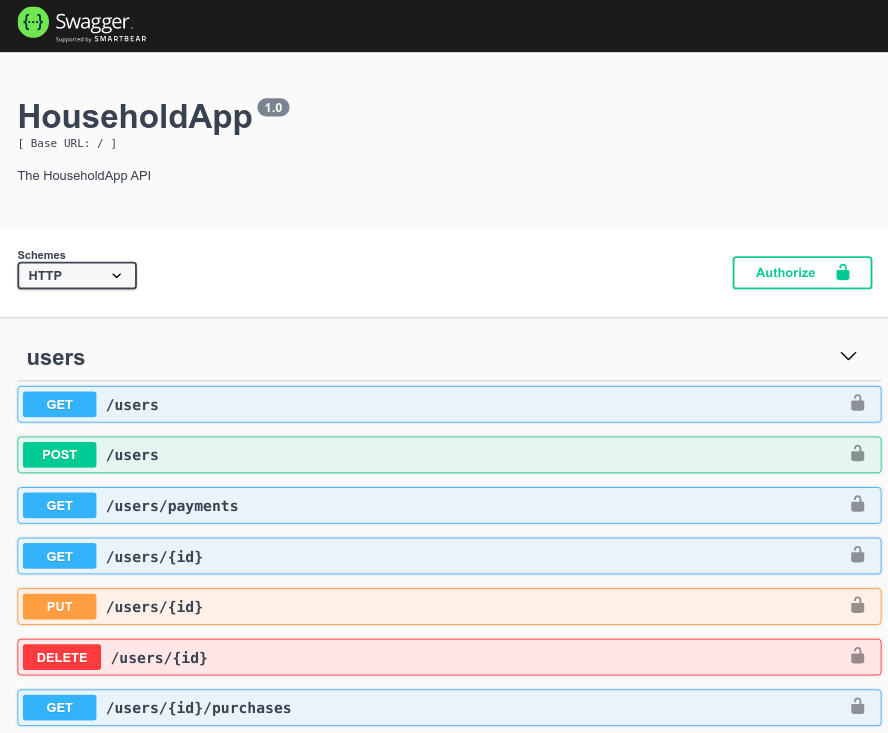
\includegraphics[keepaspectratio,
    width=\linewidth,
    height=\dimexpr\textheight-2\baselineskip]{screenshots/swagger_1.png}
  \caption{Swagger - widok struktury RESTapi.}
  \label{ss:swagger_gui}
\end{figure}


\begin{figure}[H]
  \centering
  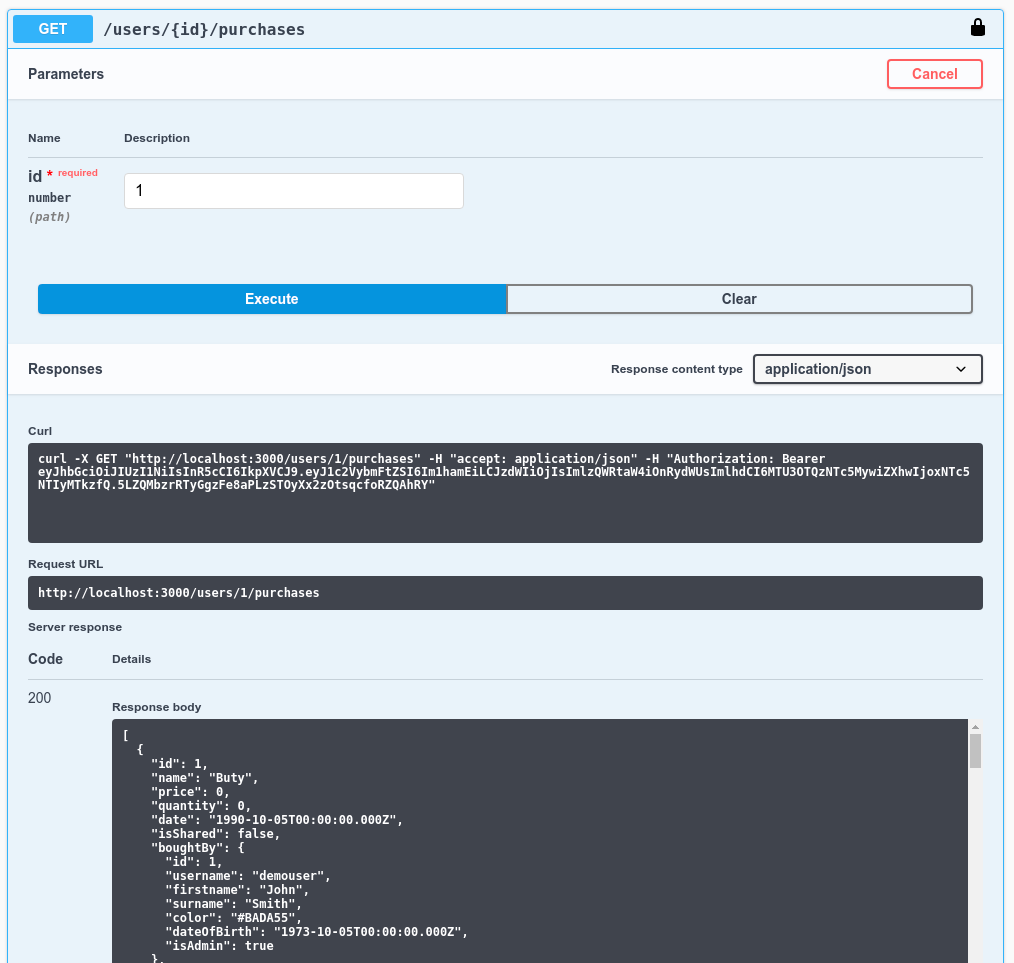
\includegraphics[keepaspectratio,
    width=\linewidth,
    height=\dimexpr\textheight-2\baselineskip]{screenshots/swagger_2.png}
  \caption{Swagger - wywołanie punktu końcowego.}
  \label{ss:swagger_query}

\end{figure}



% Swagger wisienką na torcie https://docs.nestjs.com/recipes/swagger

\newpage
\subsection{Frontend}
Interface użytkownika został napisany używając frameworka SPA VueJs. Za wygląd i funkcjonowanie komponentów odpowiedzialny był framework Vuetify, który dostarcza komponenty w stylu Material Design.

\subsubsection{Routing i podstawowe ścieżki}

Aplikacja posiada dwa zagnieżdżone routery. Pierwszy steruje głównym widokiem i przełącza pomiędzy widokiem logowania, a widokiem pozostałej części aplikacji. Drugi z nich, zawarty w widoku aplikacji, odpowiada za przełączanie widoku aplikacji pod wpływem wybieranie pozycji z menu. Listing \ref{lst:init} przedstawia kod inicjujący aplikację poprzez podanie obiektów konfiguracyjnych routera, store'a, Vuetify oraz funkcji renderującej, która jako argument przyjmuje główny komponent aplikacji - \lstinline{App}

\begin{lstlisting}[language=JavaScript, caption={Punkt wejścia skryptu inicjującego aplikację.}, label=lst:init]
import App from "./App.vue";
import router from "./router";
import store from "./store";
import vuetify from "./plugins/vuetify";
new Vue({
  router,
  store,
  vuetify,
  render: h => h(App)
}).$mount("#app");
\end{lstlisting}

Rysunek \ref{ss:login} i \ref{ss:dashboard} przedstawiają kolejno stronę logowania i pozostałą część aplikacji. Obszarem działania zagnieżdżonego routera jest obszar prawej części ekranu na rysunku \ref{ss:dashboard}.

\begin{figure}[H]
  \centering
  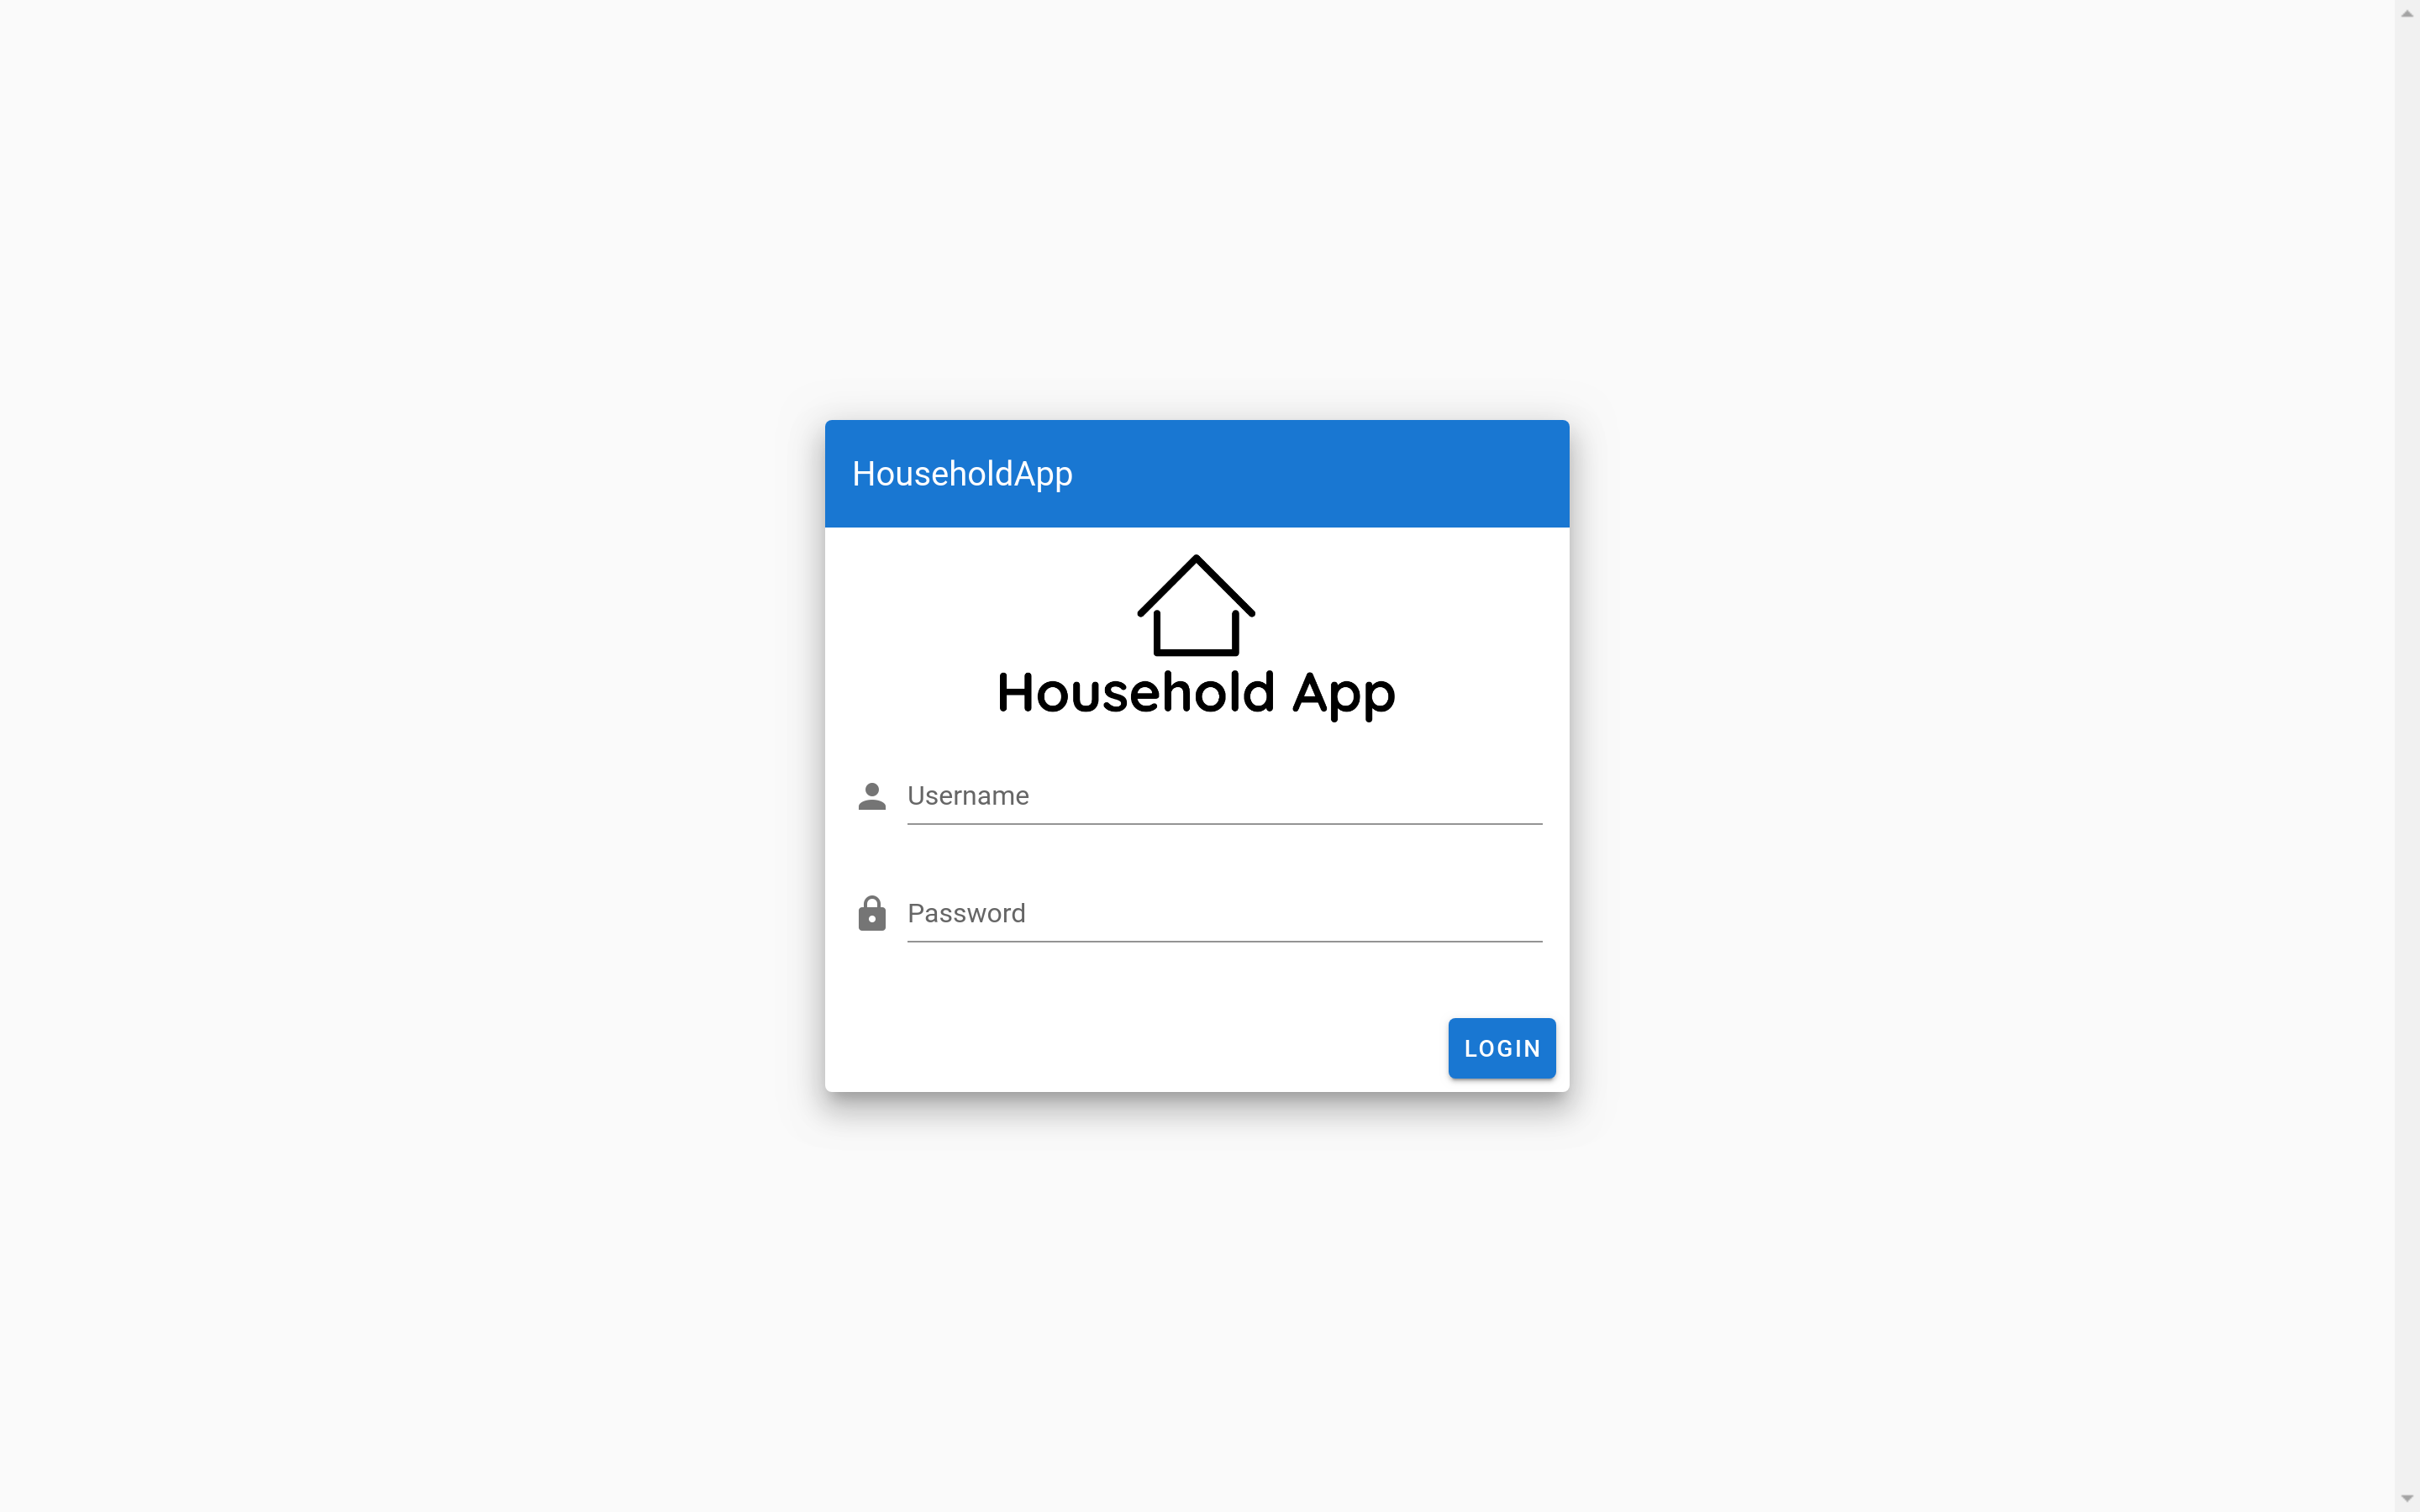
\includegraphics[width=0.95\linewidth]{screenshots/login}
  \caption{Widok strony logowania (\lstinline{/login}).}
  \label{ss:login}
\end{figure}
\begin{figure}[H]
  \centering
  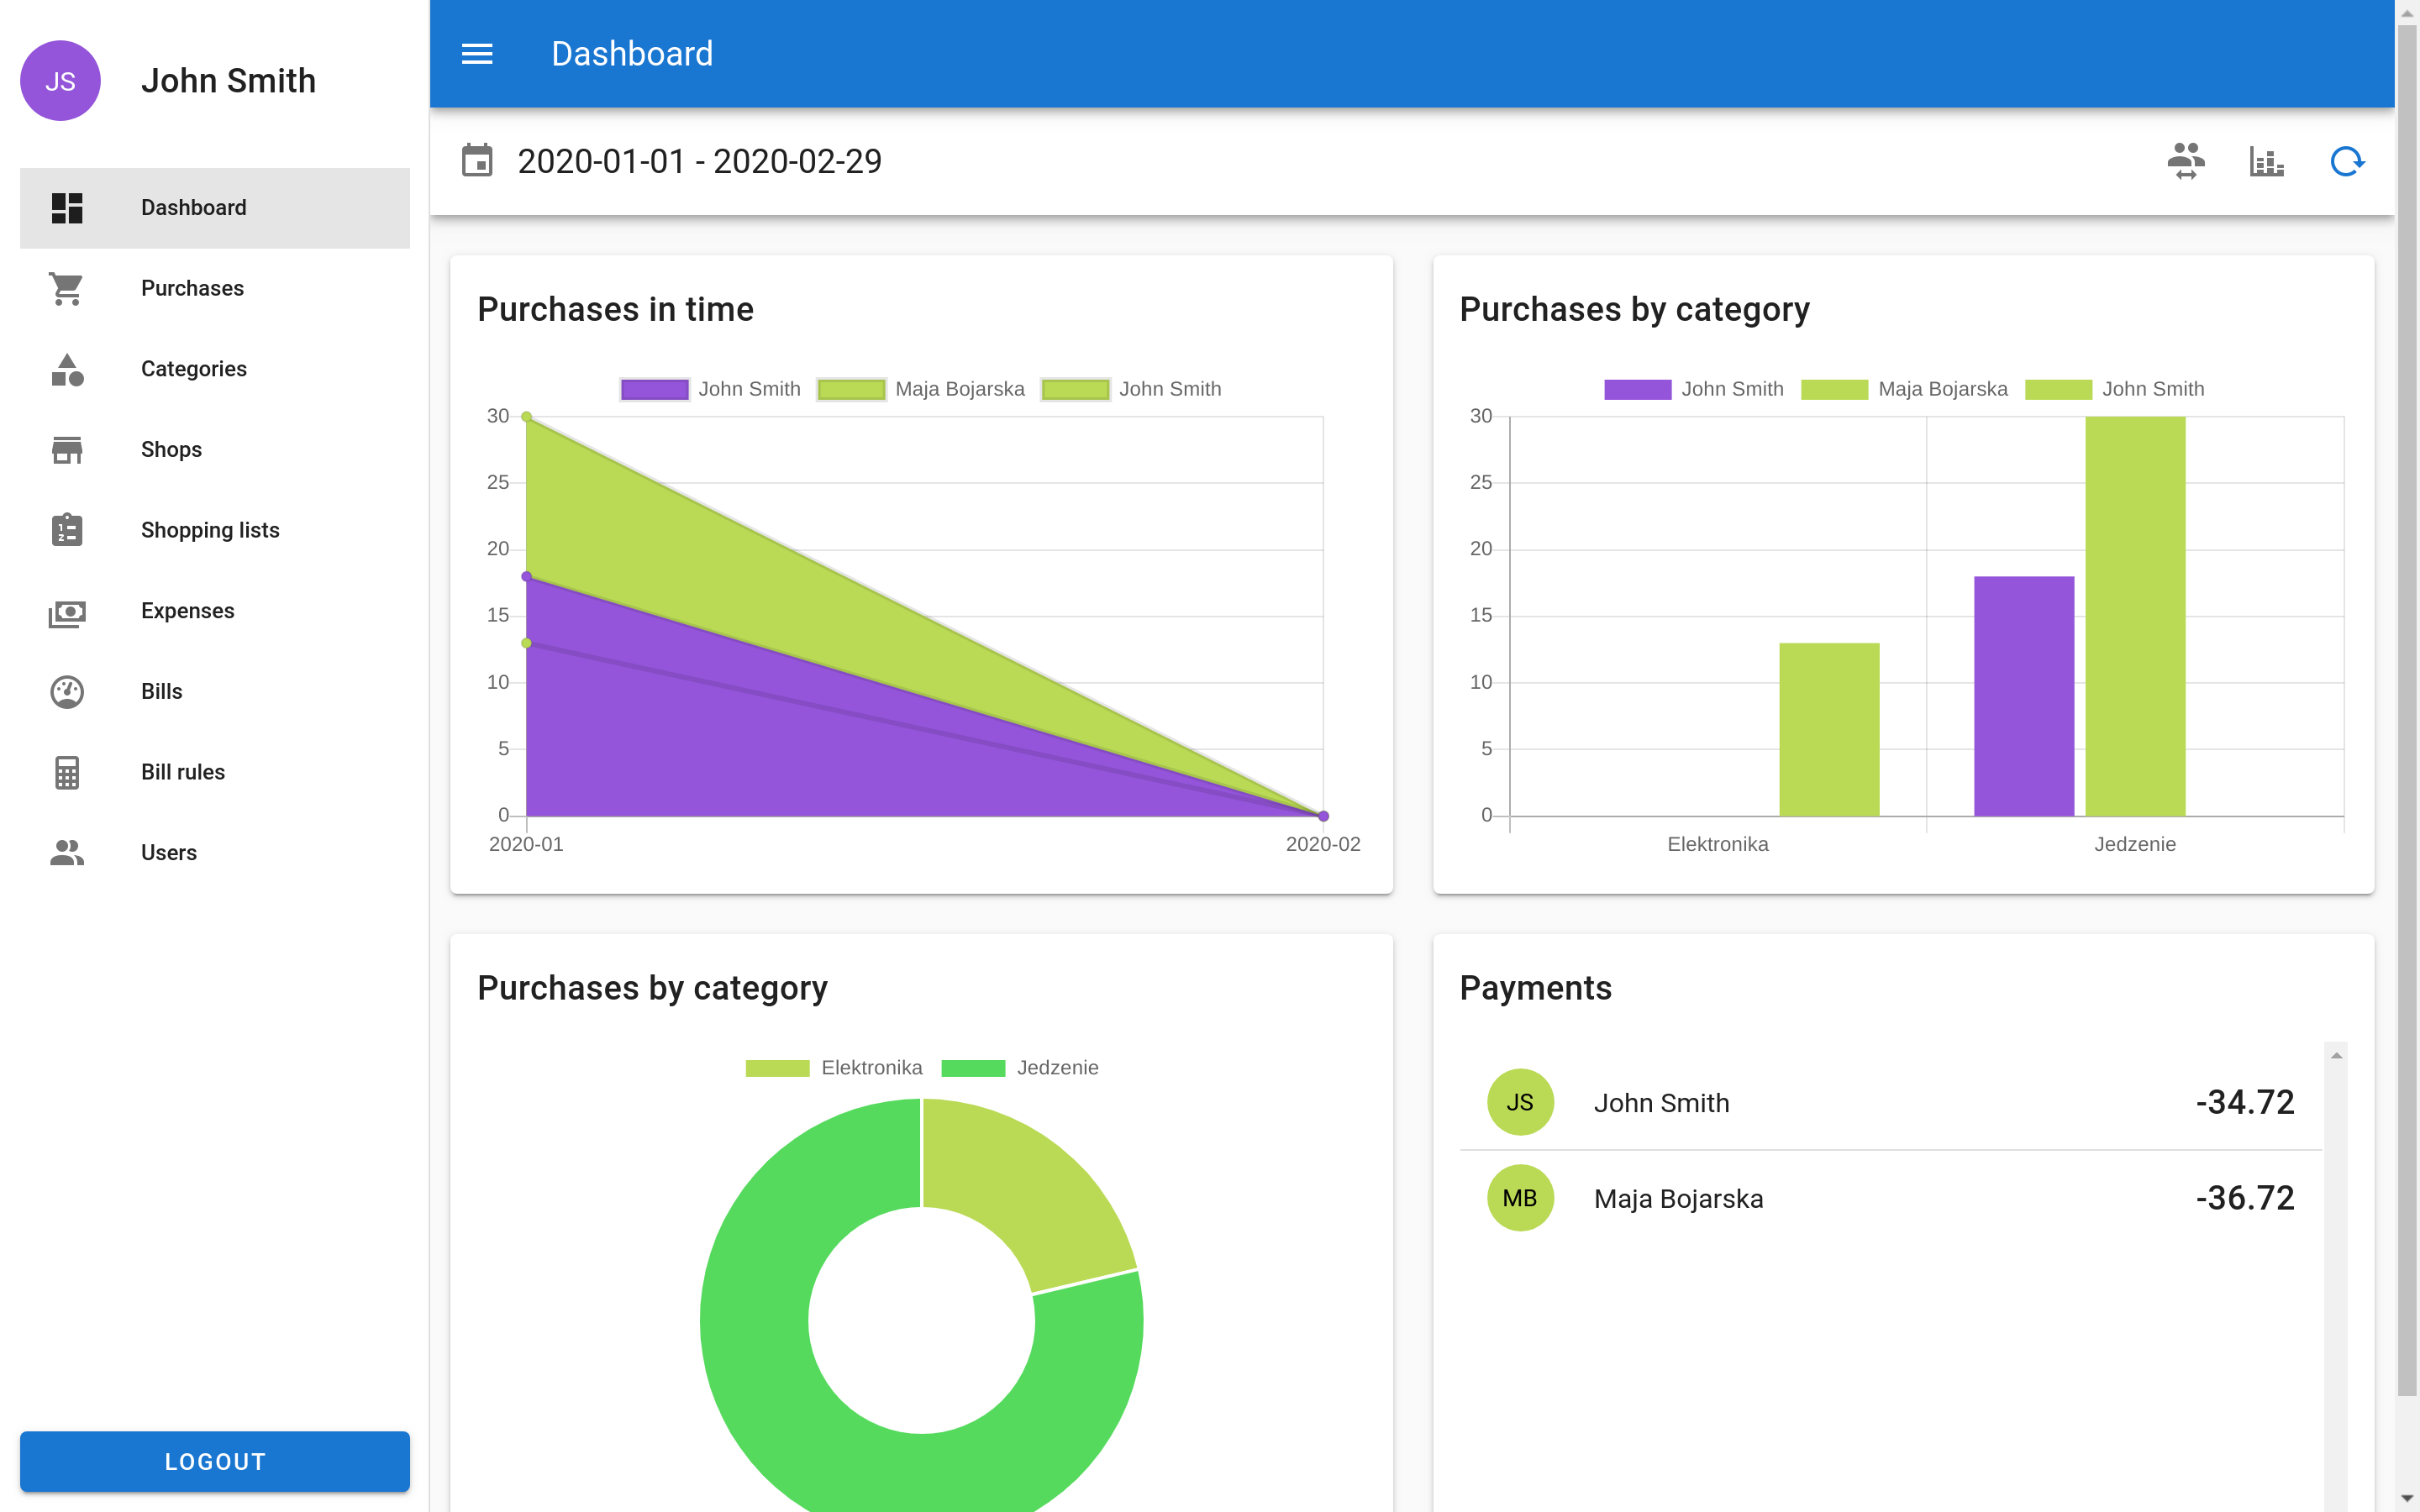
\includegraphics[width=0.95\linewidth]{screenshots/dashboard}
  \caption{Widok podsumowania (\lstinline{/dashboard}).}
  \label{ss:dashboard}
\end{figure}

\subsubsection{Komunikacja z serwerem}

Do konfiguracji z serwerem wykorzystana została biblioteka \lstinline{Axios}, która po konfiguracji adresu i portu wysyłała zapytania HTTP. Konfigurację i przykładowe zapytania zamieszczono na listingu \ref{lst:axios}.
\begin{lstlisting}[language=JavaScript, caption={Axios - konfiguracje i przykładowe użycie.}, label=lst:axios]
axios.defaults.baseURL = `http://${process.env.VUE_APP_API_URL}:${process.env.VUE_APP_API_PORT}`;
...
axios
  .get("expenses", { headers: { Authorization: this.authHeader } })
  .then((response: AxiosResponse) => {
    this.expenses = response.data;
  });
\end{lstlisting}

Na listingu \ref{lst:axios} widać również przekazywanego z każdym zapytanie wymagającym uwierzytelnienia nagłówka \lstinline{Authorization} o treści \lstinline{Bearer <TOKEN>}, gdzie \lstinline{<TOKEN>} jest tokenem otrzymanym wcześniej w procesie uwierzytelniania.

\subsubsection{Wyświetlanie i edycja danych}

Dane wyświetlane są w postaci list (rysunek \ref{ss:list}). Pozycję z listy można dodać i edytować za pomocą komponentu formularza, który pojawia się na ekranie jako okno dialogowe (rysunek \ref{ss:dialog}).

\begin{figure}[H]
  \centering
  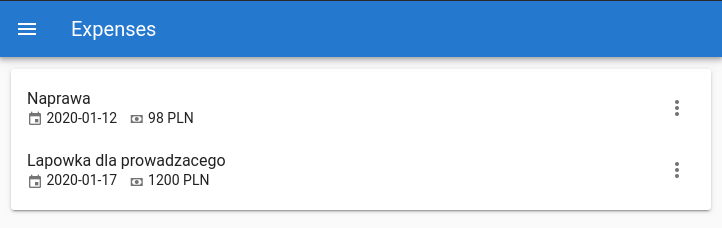
\includegraphics[width=0.8\linewidth]{screenshots/list}
  \caption{Lista wydatków (\lstinline{/expenses}).}
  \label{ss:list}
\end{figure}
\begin{figure}[H]
  \centering
  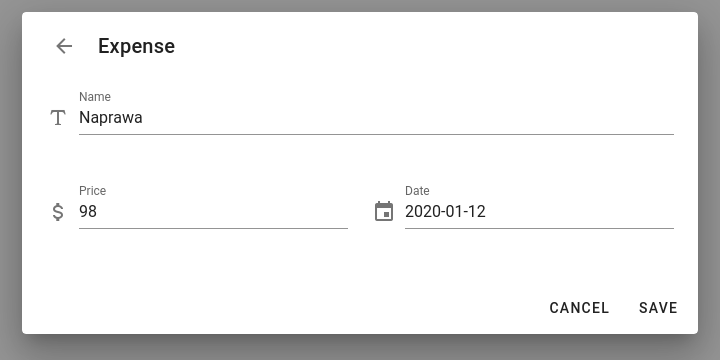
\includegraphics[width=0.8\linewidth]{screenshots/dialog}
  \caption{Edycja wydatku (\lstinline{/expenses}).}
  \label{ss:dialog}
\end{figure}

Widok listy, z pominięciem danych, definiowany jest w szablonie komponentu pokazanym na listingu \ref{lst:list}. Komponenty frameworka Vuetify charakteryzuje prefix \lstinline{v-}. Na owym listingu widać również osadzony komponent \lstinline{expense-form}, który wyświetlany jest jako ciało okna dialogowego.

\begin{lstlisting}[language=HTML, caption={Struktura widoku listy z pominięciem wyświetlania danych.}, label=lst:list]
<template>
  <v-container>
    <v-card v-if="expenses.length > 0">
      <v-list>
        <v-list-item v-for="expense in expenses" :key="expense.id"
          @click.stop="edit(expense)" >
          <v-list-item-content>
            <v-list-item-title>...</v-list-item-title>
            <v-list-item-subtitle>...</v-list-item-subtitle>
          </v-list-item-content>
          <v-list-item-action @click.stop>...</v-list-item-action>
        </v-list-item>
      </v-list>
      <v-snackbar v-model="snackbarVisible">...</v-snackbar>
    </v-card>
    <v-card v-else>...</v-card>
    <v-dialog
      v-model="dialogVisible" 
      max-width="800px"
      :fullscreen="$vuetify.breakpoint.xsOnly"
    >
      <expense-form
        :expense="dialogExpense"
        @close="dialogVisible = false"
        :type="formType"
        @submit="submit"
      />
    </v-dialog>
    <v-btn @click="create" color="primary" fab fixed right bottom>
      <v-icon>mdi-plus</v-icon>
    </v-btn>
  </v-container>
</template>
\end{lstlisting}

\subsubsection{Walidacja danych}
Za walidację danych odpowiedzialny jest komponent \lstinline{v-form}, którego obiekt posiada metodę \mbox{\lstinline{validate()}}. Walidacja wykonuje się również po każdorazowej zmiany wartości pól formularza. Komponent analizuje wartość wszystkich komponentów-dzieci wykonując na nich zdefiniowane przez aplikację reguły. Są one zdefiniowane jako jako funkcje, przyjmujące jako argument wartość pola i zwracające wartość \lstinline{true} przy poprawnej jego wartości, albo ciąg znaków z komunikatem błędu. Metodę \lstinline{validate()} odpowiedzialna jest również za wyświetlanie komunikatów użytkownikowi.
Listing \ref{lst:validation} pokazuje użycie komponentu pola tekstowego, a listing \ref{lst:validationRules} rozwinięcie reguły jego walidacji. Rysunek \ref{ss:validation} przedstawia komunikat błędu walidacji.

\begin{lstlisting}[language=HTML, caption={Komponent pola tesktowego}, label=lst:validation]
<v-text-field
  v-model="editExpense.name"
  label="Name"
  prepend-icon="mdi-format-text"
  :rules="rules.required"
/>
\end{lstlisting}
\newpage
\begin{lstlisting}[language=JavaScript, caption={Obiekt reguł walidacji.}, label=lst:validationRules]
readonly rules = {
  required: [(v: string) => !!v || "Field is required!"]
};
\end{lstlisting}

\begin{figure}[H]
  \centering
  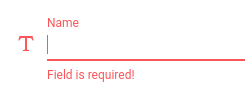
\includegraphics[width=0.3\linewidth]{screenshots/validation}
  \caption{Walidacja pola tekstowego danych edycji wydatku (\lstinline{/expenses}).}
  \label{ss:validation}
\end{figure}

\subsubsection{MVVM - Model, View, ViewModel}
Każdy komponent widoku i formularza w swojej klasie posiada zdefiniowane pola, które zawierają wyświetlane i edytowalne pola obiektów. Przykładem tego jest komponent widoku \lstinline{Expenses}, który zawiera tablicę obiektów \lstinline{Expence}. Obiekty te stanowią model widoku (ViewModel). Obiekty klas odpowiedzialne za działanie tych komponentów pośredniczą w wymianie danych pomiędzy widokiem, czyli wyświetlanym formularzem bądź listą, a modelem widoku (View <-> ViewModel). Modelem w tej relacji jest encja zapisana w bazie danych i synchronizowana a modelem widoku w momencie wywołania zdarzeń zapisania i odczytania danych z serwera \cite{mvvm}.